\section{Data Visualization}
%\begin{frame}[fragile]
%  \frametitle{Data Visualization}
%  \framesubtitle{\texttt{import Gnuplot}}
%\end{frame}

\begin{frame}[fragile]
  \frametitle{Data Visualization}
  \framesubtitle{\texttt{import matplotlib}}
    \lstset{tabsize=2, language={Python}, basicstyle=\normalsize\ttfamily,
      keywordstyle=\color{blue}, rulesepcolor=\color{black},
      captionpos=bi, breaklines=true, escapechar=*, upquote=true,
      commentstyle=\color{green}\ttfamily, emph={},
      emphstyle={\color{red}}}
    \begin{lstlisting}
df.head()
df = df.sort('probe_count', ascending=False)
ax = df.plot('asn_v4', 'probe_count', kind='bar')
ax.set_xlabel("ASN");
ax.set_ylabel("#Connected* Probes");
    \end{lstlisting}
    \centering
    \begin{columns}
      \begin{column}{0.45\textwidth}
        \centering
        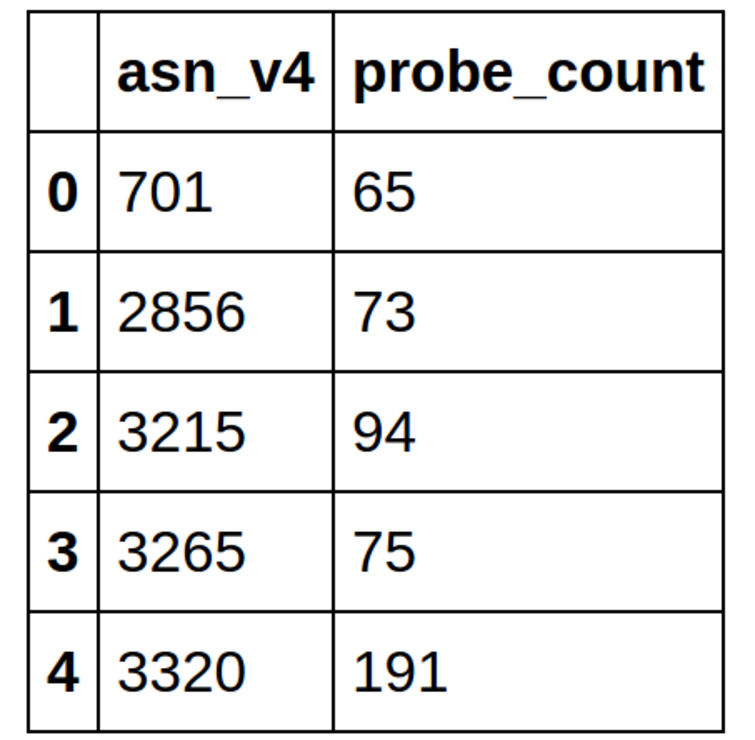
\includegraphics[width=.45\linewidth]{figures/pandas-read-sql}\\
      \end{column}
      \begin{column}{0.55\textwidth}
        \centering
    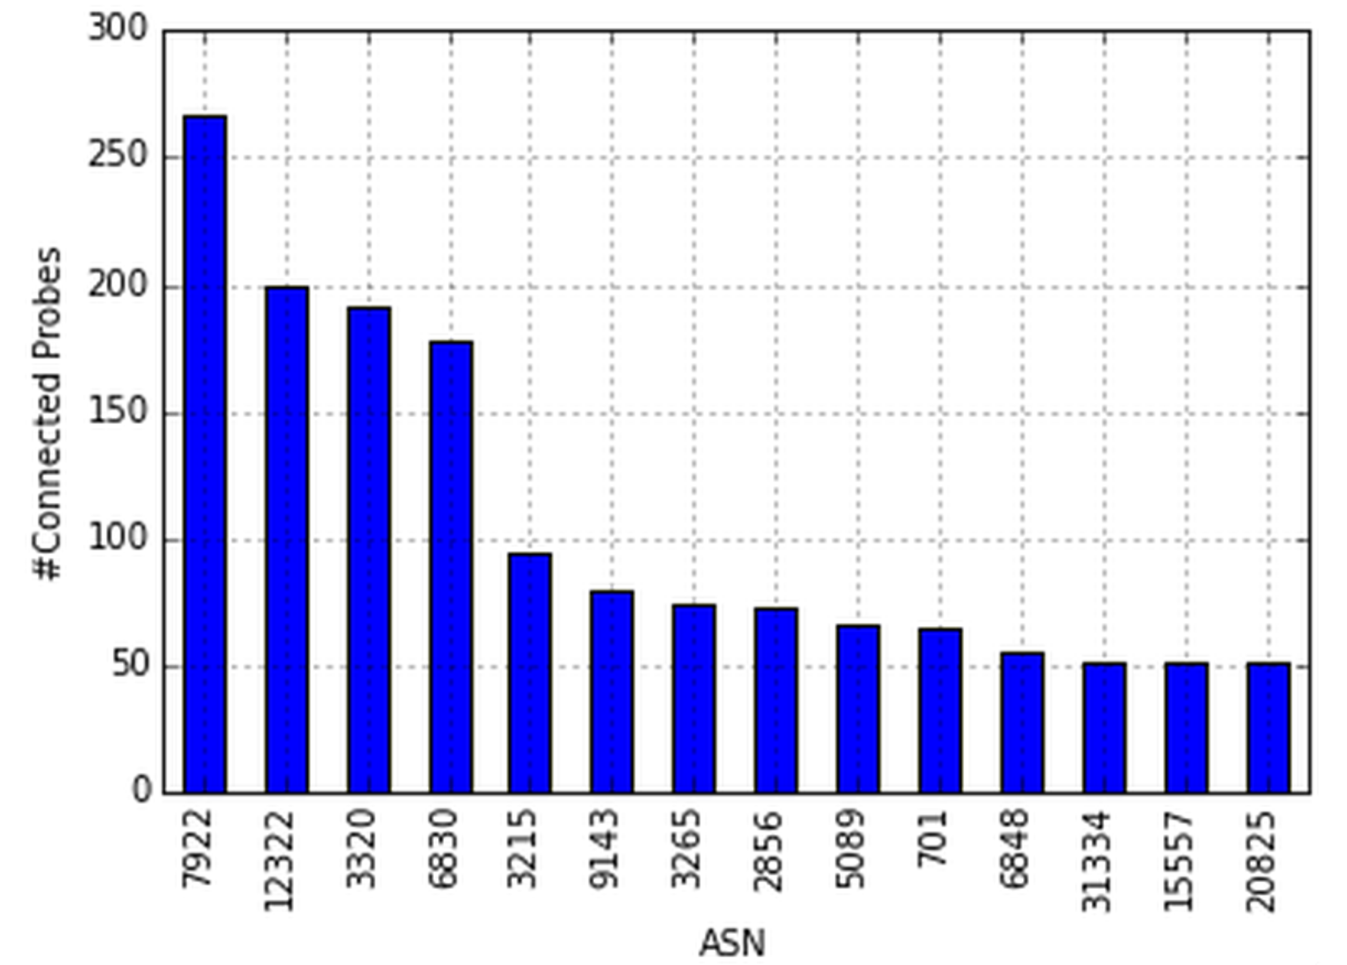
\includegraphics[width=.55\linewidth]{figures/pandas-plot}\\
      \end{column}
    \end{columns}
\end{frame}

%\begin{frame}[fragile]
%  \frametitle{Data Visualization}
%  \framesubtitle{\texttt{graphviz}}
%\end{frame}

%\begin{frame}[fragile]
%  \frametitle{Data Visualization}
%  \framesubtitle{\texttt{d3.js}}
%\end{frame}
